\section*{Desarrollo}
En esta secci\'on se podran observar los pasos para el diseño del filtro y el detalle de los c\'alculos empleados para lograr el comportamiento requerido, junto con las prubeas y respuestas en frecuencia pedidas.\\

%---------------------------------------------------------------%

\subsection*{Problema a resolver}
El filtro a diseñar vino dado por la siguiente ecuaci\'on de transferencia. \\
\begin{equation}
	H(s)=\frac{s^2}{s^2+3510 . s+1.004\times10^7}	
\end{equation}


Esta transferencia es la n\'umero 4, de la lista provista en clase.
Por la forma de la ecuaci\'on, se observa que se trata de un filtro del tipo \textit{Pasa Altos}. Esto es, haciendo limite con $s \rightarrow +\infty$, resulta una amplifiacion de 0\dB \ y se tiene un atenuaci\'on infinita para $s\rightarrow-\infty$.

\subsection*{Diseño del filtro}
Se identificaron los par\'ametros de la transferencia del filtro a partir de la forma de Bode vista en clase.\\

\begin{equation}
  H(s)=H_0\ \frac{s^2}{s^2 +s \frac{\omega_0}{Q} +\omega_0^2}
\end{equation}
De la consigna se obtiene que la frecuencia de corte es 
$\omega_0=\sqrt{1.004\times10^7}=3169$, por lo que $f_0=\frac{\omega_0}{2\pi}=504\Hz$. Con este dato, encontramos que $Q=\frac{\omega_0}{3510}=0.902$.\\
Ademas, la transferencia tiene un cero doble en $C_0=0$ y polos complejos conjugados en $p_{0,1}= -1755\pm j\ 2638 $. La forma compeja de los polos es coherente al tener $Q>0.5$.
Por ultimo, $H_0 =1$  ya que no hay amplificacion superada la frecuencia de corte.\\
\pagebreak
%---------------------------------------------------------------%

\subsection*{Diagramas de Bode}
Para la transferencia hallada, se realizaron los diagramas de Bode en el software \texttt{Matlab} de calculo num\'erico. Definiendo a $s$  como una variable de transferencia y con la funcio\'on \textit{bode()} se obtuvo la siguiente figura\\
%\pagebreak
\begin{figure}[h]
	\centering
	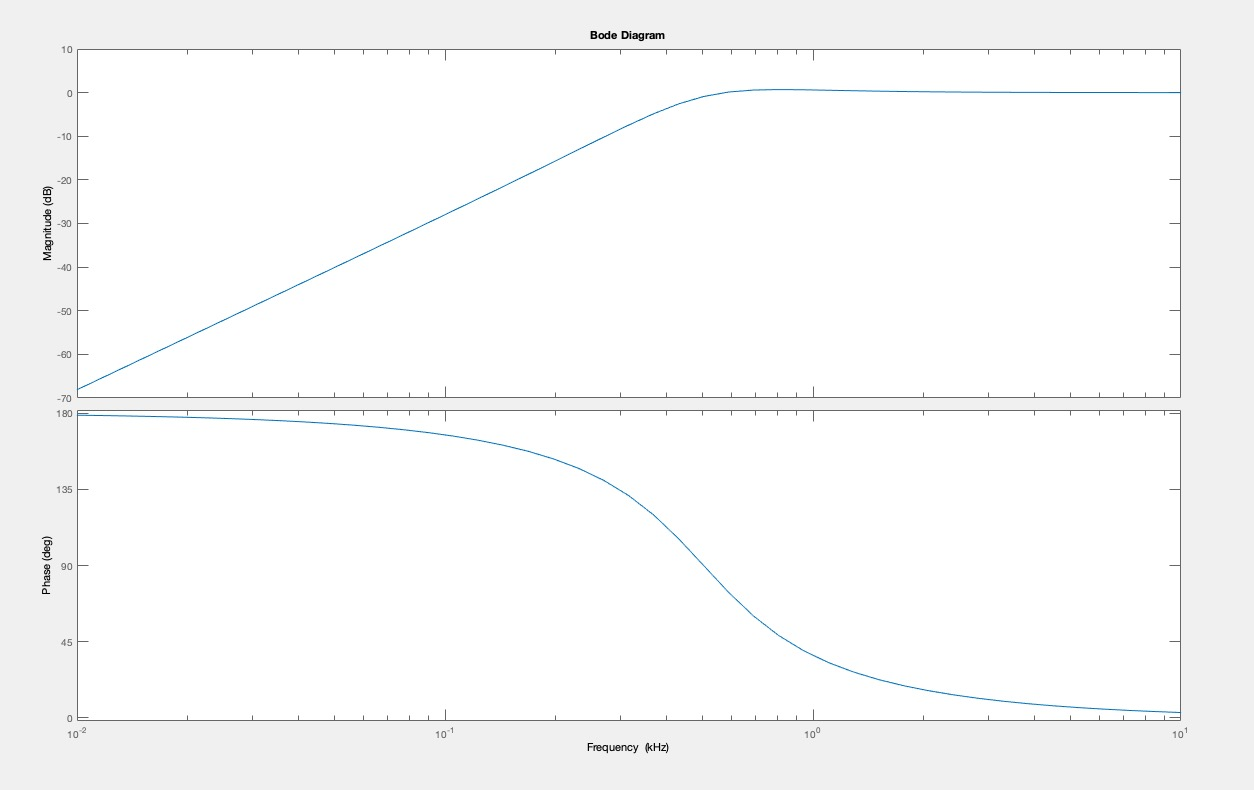
\includegraphics[width=18cm]{imagenes/BODE.jpg}	\caption{Diagrama de Bode teorico en Matlab}
\end{figure}

Se puede apreciar el comportamiento de \textit{Pasa Altos} y tambien que est\'a aplicado a la frecuencia correcta ($\sim 500\Hz$). Luego viendo el nivel de amplificacion para las altas frecuencias, se observa un nivel de $0 \dB$, lo cu\'al coincide con el esperado.

%---------------------------------------------------------------%
\subsection*{Respuesta del filtro teorico a distintas señales}

Luego del diagrama de Bode, se realizaron graficos donde se muestran qu\'e salida tiene el filtro dada una señal de entrada como: \textit{escal\'on}, \textit{impulso} y \textit{cuadrada}.\\

Para la respuesta a la señal cuadrada, se eligieron tambien,  3 frecuencias acordes, $f_1 = \frac{f_0}{10}=50,4 \Hz$, $f_2 = f_0 = 504\Hz$, $f_3 = 10.f_0= 5,04 \kHz$.
Se lograron los siguientes resultados.\\

%TODO: LLEGUE HASTA ACA, FALTA PONER GRAFICOS NUEVOS MAS LEGIBLES Y CONTINUAR DESCRIPCIONES%

\begin{figure}[hbt]
	\centering
	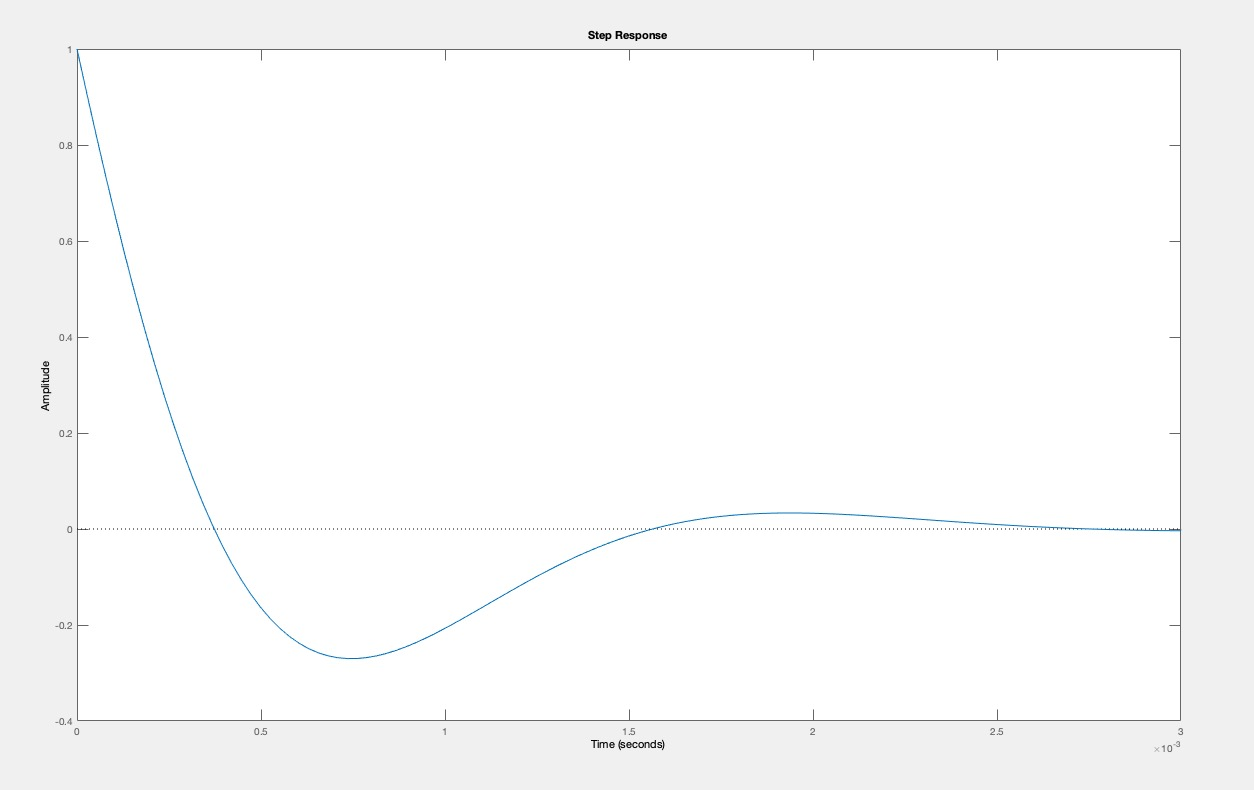
\includegraphics[width=9cm]{imagenes/STEP.jpg}
	\caption{Respuesta al escal\'on.}
\end{figure}
Se puede observar que se logra un nivel de tensi\'on estable cerca de los $6 \ms$, adem\'as, se ve que el valor al que estabiliza es $3 \V$, que es acorde a la  amplificacion de $3\ veces$ o $9.54 \dB$.\\

\begin{figure}[hbt]
	\centering
	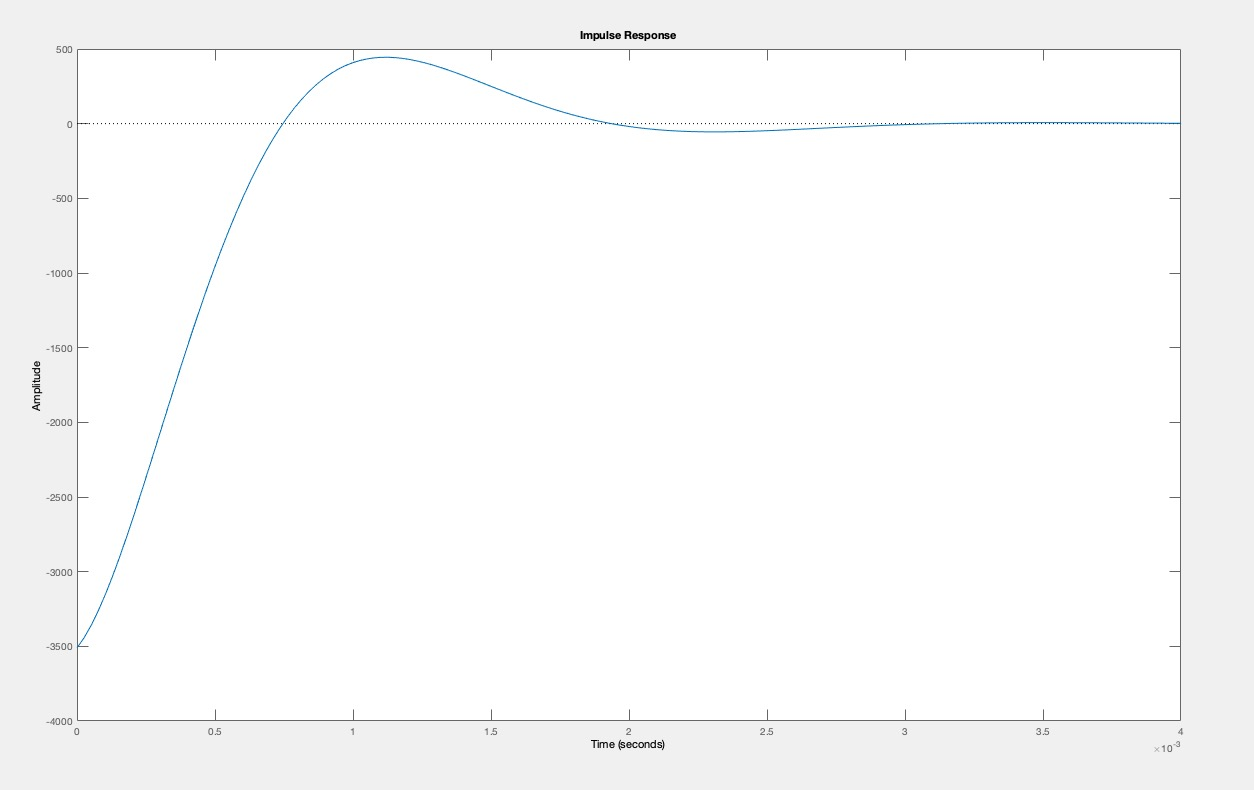
\includegraphics[width=8cm]{imagenes/IMPULSE}	\caption{Respuesta al impulso.}
\end{figure}
Aqui se observa que existe mucha mas variaci\'on de tensi\'on en el transitorio hasta los $3 \V$, que se alcanzan en $5 \ms$.\\

\begin{figure}[hbt]
	\centering
	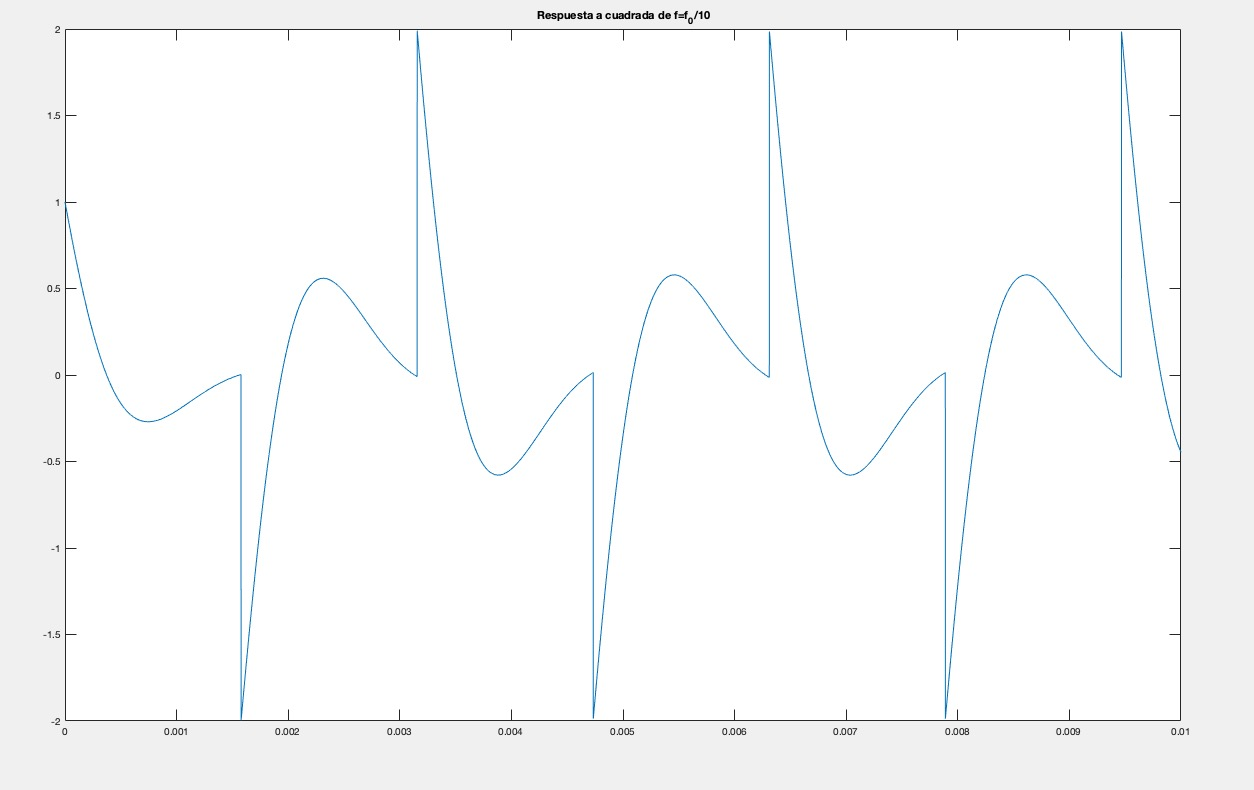
\includegraphics[width=8cm]{imagenes/sen f:10.jpg}	\caption{Respuesta a una señal senoidal de $10\Hz$}	
\end{figure}

Se observa que la señal representada con color azul es la salida  y el color gris es la señal de entrada. Notar la amplificacion a $3\V$ y que la señal no sufre atenuaci\'on visible, resultado esperable para esta frecuencia.\\

\begin{figure}[!h]
	\centering
	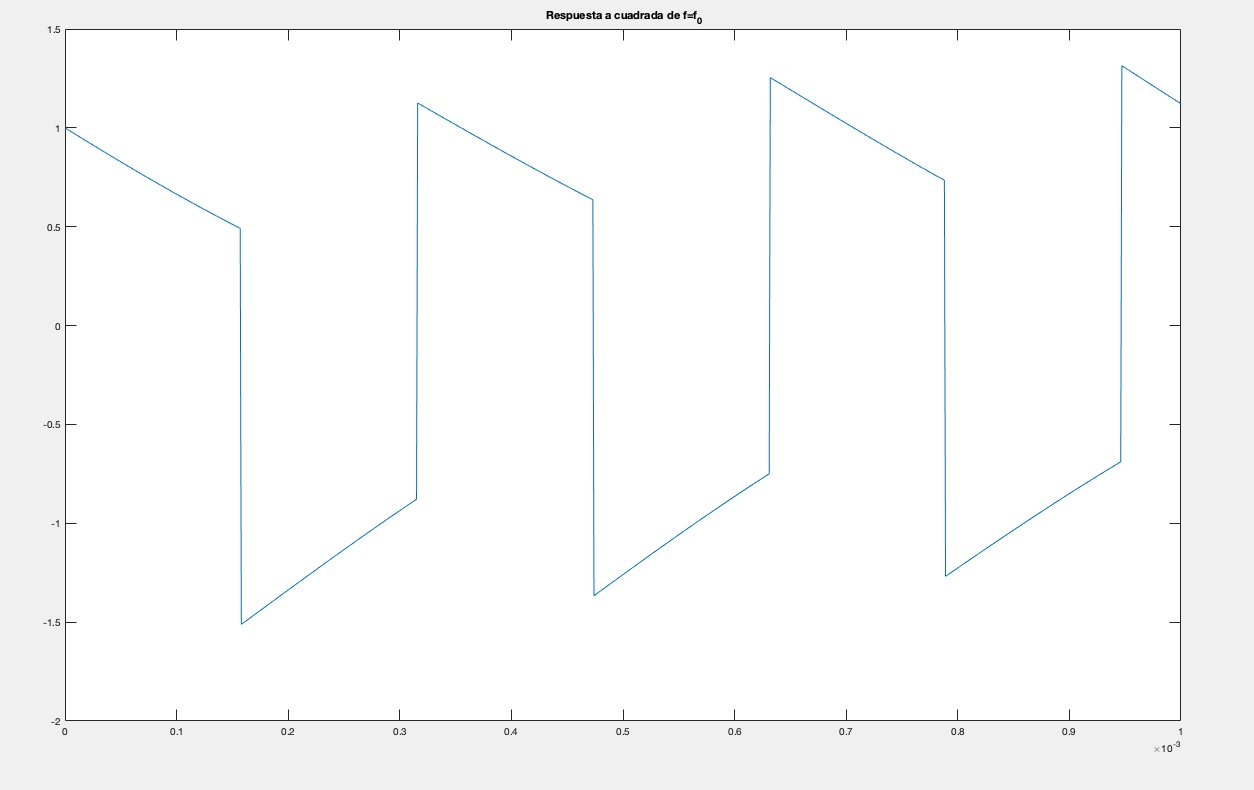
\includegraphics[width=8cm]{imagenes/sen f.jpg}	\caption{Respuesta a una señal senoidal de $1\kHz$}	
\end{figure}

Aqui observamos que la salida sufre una gran atenuacion luego del transitorio, tanto que se puede considerar como de amplitud nula. Aqui se ve claramente el efecto de \textit{elimina-banda}, donde el filtro se encarga de que la señal no tenga amplitud apreciable si su frecuencia es de $1\kHz$.\\
Como ultimo comentario, la atenuaci\'on es total dado que la entrada es de tipo senoidal y estas funciones no estan compuestas por otras de distinta frecuencia,  como si es el  caso en señales triangulares o cudradas.\\

\begin{figure}[!h]
	\centering
	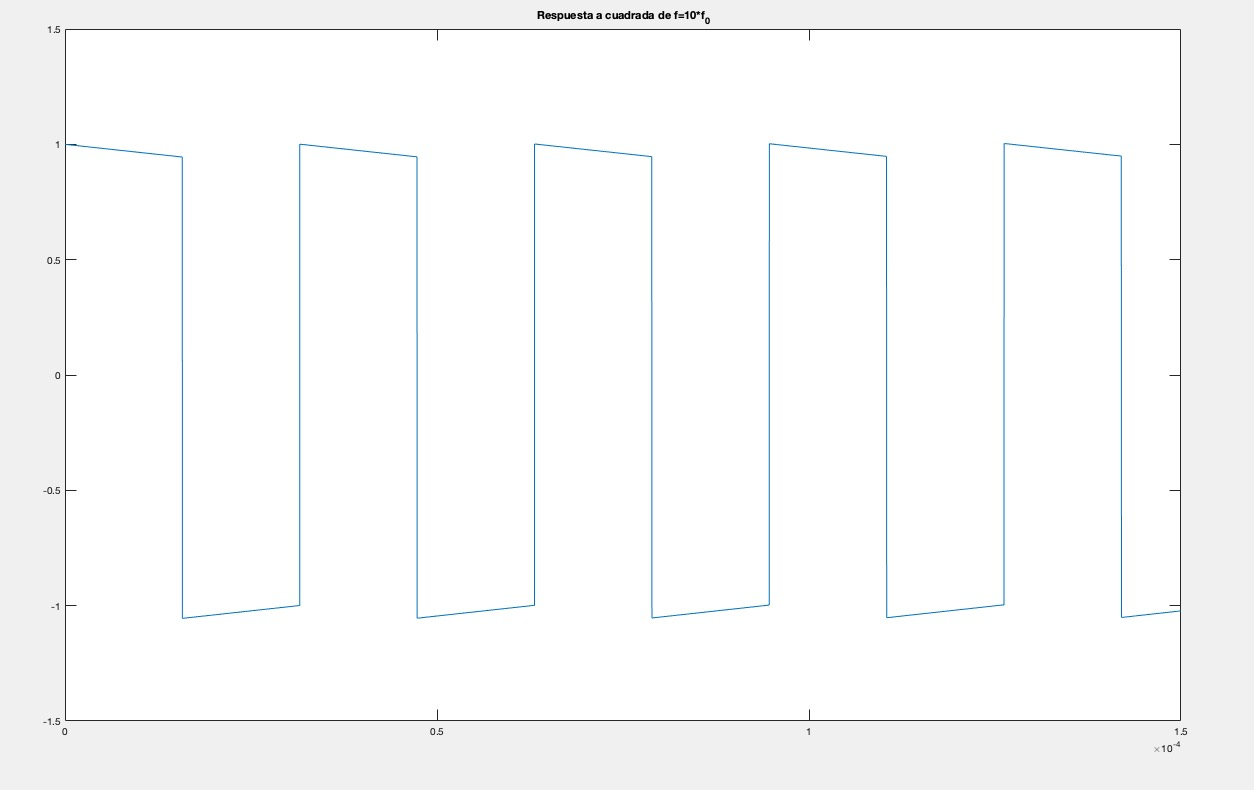
\includegraphics[width=8cm]{imagenes/sen 10f}	\caption{Respuesta a una señal senoidal de $100\kHz$}	
\end{figure}
En esta respuesta, se ve un efecto similar a la respuesta a la senoidal de $10\Hz$, donde se ve un nivel de  amplificacion hasta los $3\V$ y la  señal no sufre atenuaci\'on visible.\\

\begin{figure}[hbt]
	\centering
	\includegraphics[width=8cm]{imagenes/}	\caption{Respuesta a una señal senoidal de $100\Hz$}	
\end{figure}

Se observa la salida a una señal cuadrada de $100 \Hz$, notar que el circuito responde muy similar al escal\'on, esto se debe a la baja frecuencia de esta señal, que tiene un per\'iodo mucho mas bajo que el tiempo caracteristico del circuito.

\begin{figure}[hbt]
	\centering
	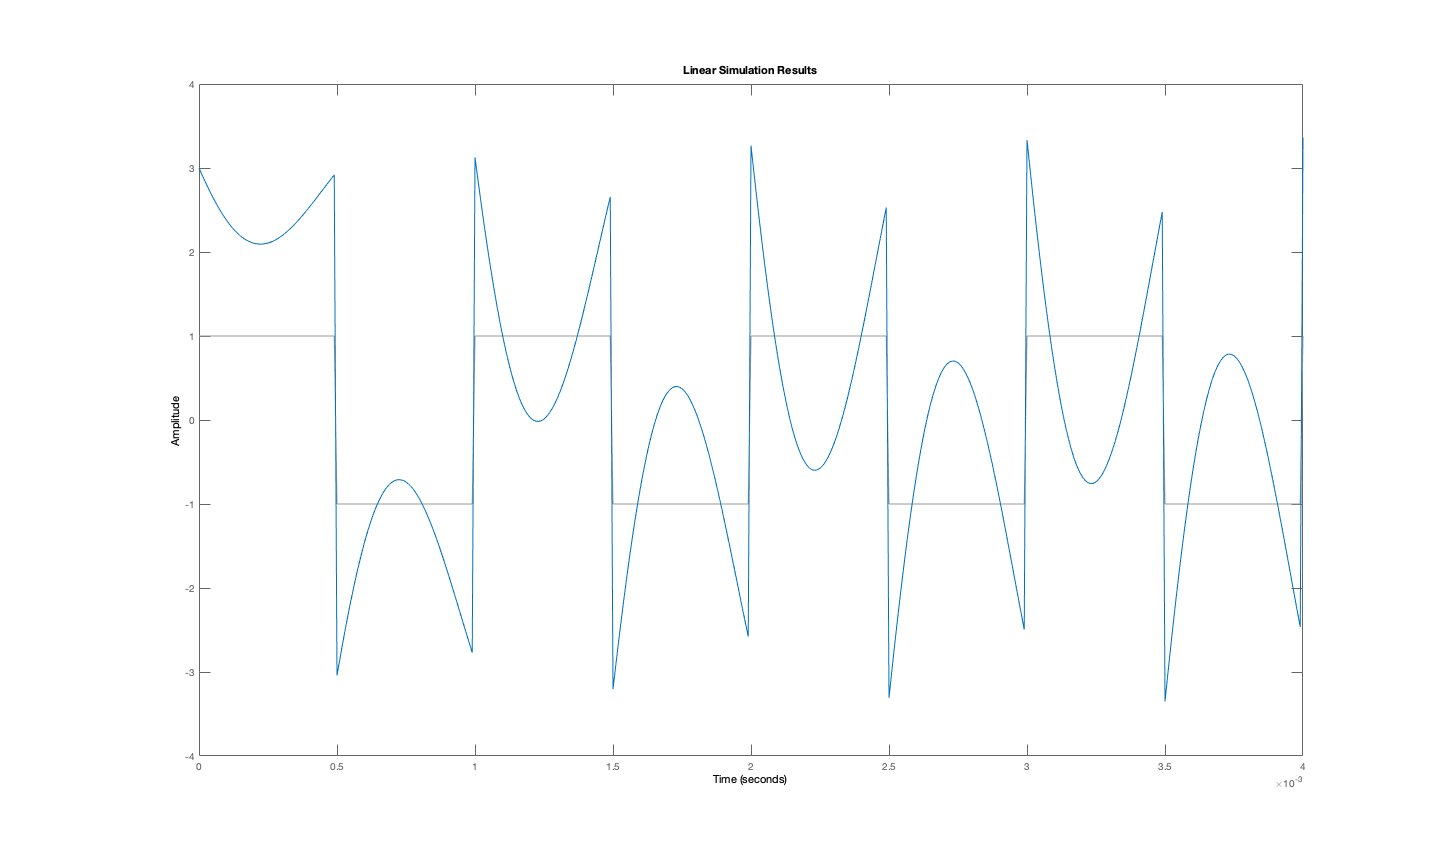
\includegraphics[width=8cm]{imagenes/rtasqar1k}	\caption{Respuesta a una señal senoidal de $1\kHz$}	
\end{figure}
En esta salida se observa una variaci\'on en la salida cada vez mas grande a medida que el tiempo avanza, con caracteristicas de oscilaci\'on muy predominantes.\\

\pagebreak
\begin{figure}[hbt]
	\centering
	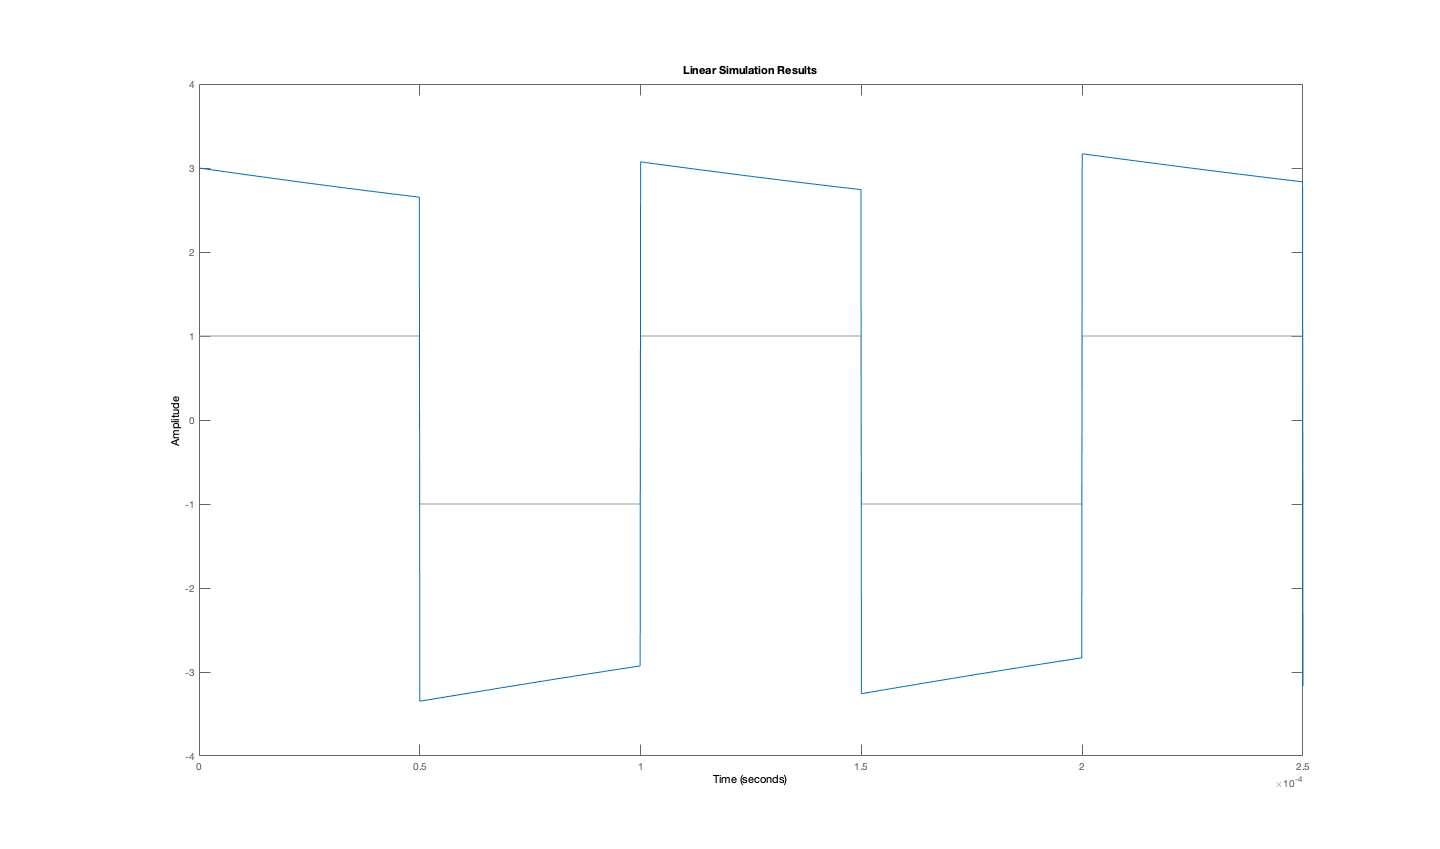
\includegraphics[width=8cm]{imagenes/rtasqar100k}	\caption{Respuesta a una señal senoidal de $100\kHz$}	
\end{figure}
Aqui se observa que la salida es menos oscilante que la anterior (sin considerar la  naturaleza oscilatoria de la señal de entada)
y que presenta una distorsion leve en cada semiciclo.

%---------------------------------------------------------------%

\subsection*{Circuito}
Se utiliz\'o el siguiente circuito:

\begin{figure}[H]
\begin{center}
\begin{circuitikz} [american,scale=0.6,transform shape]
\draw
%capacitores y entrada
(0,0) node[left] {$v_i$} to [short,o-] (1,0)
	to[C,l=$C_1$] (4,0) -- (5,0)
	to[C,l=$C_2$] (7,0)-- (8,0)
;
\draw
%opamp
(9,0.49) node[op amp] (opamp) {}
(opamp) node[] {U1}
(opamp.-) to [short,-o] (7.8,3) -- (10.2,3) to [short,-o]
(opamp.out) to [short,-o] (11,0.49) node[right] {$v_o$}
;
\draw
%R1
(4.5,0) to [short,o-] (4.5,3)
	to[R,l=$R_1$] (7.75,3)
;
\draw
%R2
(7.5,0) to  [short,o-] (7.5,-1)
	to[R,l=$R_2$] (7.5,-4)--(7.5,-5) node[ground]{}; 
;
\end{circuitikz}
\end{center}
\caption{Circuito de filtro Pasa Alto}
\end{figure}	

Aplicando el metodo de \textit{Nodos} se llega a la siguiente transferencia
\begin{equation}
  H(s) = \frac{s^2}{s^2 +s \frac{(C_1 R_1 + C_2 R_1)}{C_1 C_2 R_1 R_2}+\frac{1}{C_1 C_2 R_1 R_2}}
\end{equation}
	
Para elegir los componentes decid\'i fijar $C \defeq C_1 = C_2$ y  dejar $R_1$ y $R_2$ a determinar, dado que por la forma matematica de la transferencia, no es posible dejar ambos valores de resistencias iguales. Resulta entonces la siguiente transferencia, simplificada


\begin{equation}
  H(s) = \frac{s^2}{s^2 +s \frac{2}{C R_2}+\frac{1}{C^2 R_1 R_2}}
\end{equation}

Dadas las ecuaciones
\begin{equation}
	\frac{1}{C^2 R_1 R_2}=1,004\times10^7
\end{equation}
\begin{equation}
	\frac{2}{C R_2}=3510
\end{equation}
Resultan $R_1=5.3 \kohm$ y $R_2=17.27\kohm$,  fijando $C=33\nF$.
Por lo cual, se decidio que para armar el circuito, se utilizarian valores comerciales $R^C_1=4.7\kohm$ y para $R^C_2$ se utilizarian dos resistores de $10\kohm$ en serie, para minimizar el error en la frecuencia de corte y en factor de selectividad.

%---------------------------------------------------------------%
\subsection*{Circtuio real}
%---------------------------------------------------------------%

\subsection*{Simulaci\'on}
	Para verificar que el funcionamiento del circuito sea el esperado, se utiliz\'o el software de simulaci\'on \textit{LTSpice} con los componentes de valores comerciales. 
\begin{figure}[hbt]
	\centering
	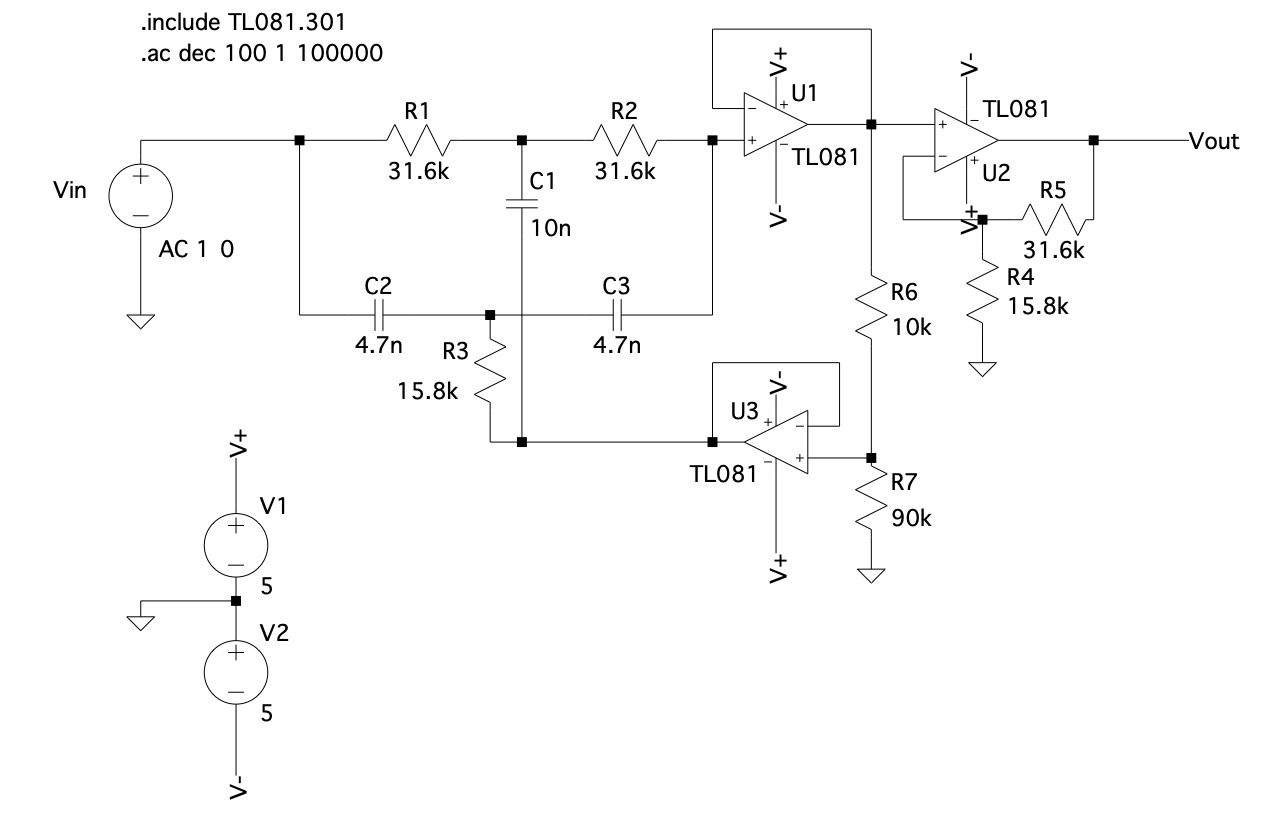
\includegraphics[width=10cm]{imagenes/simulacion}
	\caption{Circtuito simulado}
\end{figure}

	
Se utiliz\'o la directiva \texttt{.ac dec 100 1 1000000 } para
variar la  frecuencia de la fuente de entrada \texttt{ Vin } desde  $1 \si{\hertz}$ hasta $100 \kHz$. Luego se import\'o la biblioteca \textit{TL081} para el operacional. Produciendo el siguiente resultado.

%---------------------------------------------------------------%

\subsection*{Respuesta de la simulaci\'on a distintas señales}

%---------------------------------------------------------------%